\section{Ionic}

Ionic es un framework de código abierto utilizado para el desarrollo de aplicaciones hibridas para dispositivos móviles. En estos momentos se encuentra disponible la versión 2 de Ionic, que es la que vamos a usar para la realización de las prácticas que veremos en el capítulo siguiente.

Ionic funciona por encima de Apache Cordova, ayudando a conseguir que nuestras aplicaciones desarrolladas con tecnología web luzcan de cara al usuario lo más parecidas posible a las aplicaciones nativas.

Una de las características más importantes de Ionic2 es el uso que hace de Angular. Esto le permite crear aplicaciones robustas y fácilmente mantenible. El rendimiento también es otra característica fundamental. Ionic2 evita manipular el árbol DOM y hace cero uso de librerías tipo jQuery, esto unido al ya mencionado uso de Angular permite que las aplicaciones se vean realmente fluidas.

Otra facilidad que da al desarrollador, es lo que llaman Ionic Native\footnote{\url{https://ionicframework.com/docs/v2/native/}}. Esto es un conjunto de ``envoltorios'' sobre los plugins de Cordova, escritos en ES5/ES6/TypeScript y que facilitan su integración en nuestra aplicación.

Un aspecto fundamental de las aplicaciones es el apartado gráfico. Nuestra aplicación, además de funcionar bien, debe verse bien. Esto puede ser un problema ya que el mismo código deben servir para distintos tipos de terminales los cuales no comparten las mismas características de pantalla. Junto a esto, también nos enfrentamos al hecho de que cada plataforma aplica un estilo diferente a cada elemento que conforma una aplicación. Así por ejemplo, el mismo componente no se ve igual en un terminal que corra Android que uno que utilicen iOS.

\begin{figure}[htbp]
\centering
\subfigure[Android]{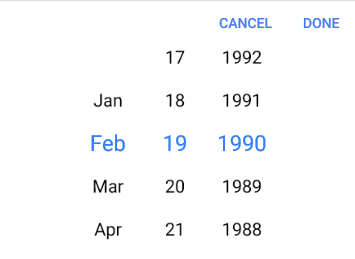
\includegraphics[width=0.45\textwidth]{Figures/ch1/ionic/date_select_android}}\hspace{0.05\textwidth}
\rulesep
\subfigure[iOS]{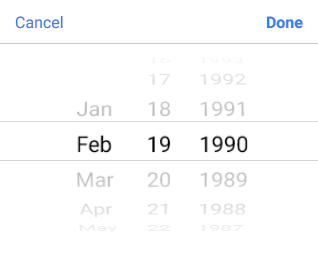
\includegraphics[width=0.45\textwidth]{Figures/ch1/ionic/date_select_ios}}
\caption{Comparación de un selector de fechas en diferentes plataformas.}
\end{figure}

Ionic ofrece un buen número de componentes\footnote{\url{https://ionicframework.com/docs/v2/components/}} que ayudan al desarrollador a enfrentarse a ambos problemas. Por otro lado, al igual que hace con Angular, Ionic implementa por debajo \gls{Sass}. \gls{Sass} es un lenguaje cuyo propósito es suplir alguna de las carencias que tiene \gls{CSS}. Cuando se compila la aplicación, los ficheros \gls{Sass} son traducidos a \gls{CSS} para que puedan ser interpretados por los navegadores. Esto es transparente para el programador, ya que es Ionic el que se encarga de realizar esta traducción.

Como ya se ha comentado, Ionic es un framework de código abierto, pudiendo hacer uso de todas sus características de forma totalmente gratuita. A parte de esto, existen cuentas de pago (se pueden consultar en \emph{https://ionicframework.com/pricing/index3.html}) para usuario o empresas que requieran un de un servicio más completo, como uso de Ionic Creator, soporte avanzado, uso de analíticas, \ldots.

También existe un ``market''\footnote{\url{https://market.ionic.io/}} en el que poder descargar temas, plugins o plantillas creados por otros usuarios (no todos los recursos son gratuitos) o compartir los nuestros con el resto del mundo. Antes de empezar a desarrollar nuestra aplicación, es recomendable revisar este market ya que podemos encontrar recursos que nos resulten útiles y evitarnos el coste de desarrollarlos ad-hoc para nuestro proyecto.

\subsection{Ionic CLI}

Ionic CLI es una herramienta que ofrece Ionic para la realización de múltiples tareas, como veremos mas adelante. Tal como la definen en la página, es como una navaja suiza a la hora de desarrollar con este framework.

La herramienta Ionic CLI se utiliza a través de la consola de comandos, indicando en el comando la acción a realizar junto con las diferentes opciones. El comando para lanzar una de estas acciones es \emph{ionic <accion>}. Cada acción tiene sus propias opciones. Muchas de estas acciones no son más que un envoltorio a herramientas propias de Cordova, como por ejemplo \emph{build}. A continuación, se va a listar estas acciones junto a sus opciones más utilizadas:

\begin{enumerate}
  \item start\footnote{url{http://ionicframework.com/docs/v2/cli/start/}}: Crea un nuevo proyecto en el directorio indicado a partir de una plantilla. Sus opciones son:
  \begin{enumerate}
    \item PATH: Directorio en el que crear el proyecto. Si no se indica, se utiliza la ruta en la que se ha ejecutado el comando.
    \item --template/-t: Plantilla a utilizar para crear la app. Se pueden ver plantillas (a las que llaman \emph{starter} en el \emph{market} de Ionic. Para utilizar una plantilla vacía, utilizar la conocida como \emph{blank}.
    \item -v2: Indica que se quiere utilizar la versión 2 de Ionic.
  \end{enumerate}
  \item serve\footnote{url{http://ionicframework.com/docs/v2/cli/start/}}: Inicia un servidor local para servir la aplicación y poder ser probada desde un navegador web. Muy útil mientras se está desarrollando.
  \item generate\footnote{url{http://ionicframework.com/docs/v2/cli/generate/}}: Comando que genera la estructura necesaria para desarrollar una nueva página o un servicio en nuestra app.
  \item platform\footnote{url{http://ionicframework.com/docs/v2/cli/platform/}}: Este comando se utiliza para manejar las plataformas a las cuales esta destinada nuestra aplicación.
  \begin{enumerate}
    \item list: Lista las plataformas y versión de estas disponible.
    \item add: Añade una nueva plataforma objetivo a nuestro proyecto.
    \item remove: Elimina una plataforma objetivo de nuestro proyecto.
  \end{enumerate}
  \item run o emulate\footnote{url{http://ionicframework.com/docs/v2/cli/run/ o http://ionicframework.com/docs/v2/cli/emulate/}}: Inicia nuestra aplicación en un terminal conectado a nuestro PC o en un emulador. Es necesario que la plataforma que utiliza este terminal/emulador se haya incluido con anterioridad al proyecto (medianto el comando anterior.
  \begin{enumerate}
    \item --livereload (en fase beta en el momento de escribir este documento): Aplica los cambios que hagamos de manera automática funcionando de manera similar a como funciona \emph{serve}. Muy útil también a la hora de depurar nuestra aplicación
  \end{enumerate}
  \item build\footnote{url{http://ionicframework.com/docs/v2/cli/build/}}: Genera una \emph{app} para la plataforma que indiquemos (al igual que ocurría con el comando anterior, la plataforma debe ser añadida previamente al proyecto), la cual es almacenada en el directorio \emph{PATH/platform}.
\end{enumerate}

\subsection{Ionic Native}
\label{subsec:IonicNative}

Ionic Native es un conjunto de envoltorios sobre los plugins de Cordova unificando en una única interfaz \gls{API} las \glspl{API} de las diferentes plataformas que soporta. Para facilitar su uso desde nuestra aplicación, implementa diferentes facilidades que ofrece Angular y TypeScript como \emph{clases} y \emph{promesas}.

Los diferentes módulos que conforman Ionic Native pueden ser instalados usando el \gls{CLI} de Ionic de manera análoga a como se instalan los plugins de Apache Cordova.

Como ejemplo, el siguiente comando se utiliza para instalar el módulo que nos permite hacer uso de la base de datos5 del dispositivo:

\begin{lstlisting}[language=bash]
  # ionic plugin add cordova-sqlite-storage
\end{lstlisting}
